\section{Introduction}
One normally surmises the presence of electronic coherence through the identification of oscillations in pump probe or 2D Electronic Spectroscopy but vibrational structure can also cause oscillations in those kinds of spectra.  Yuen-Zhou, et al\cite{witness}  in 2011 proposed a novel way of isolating electronic coherences in a system which also had vibrational structure: a pump probe spectrum performed with an impulsive laser pulse (or one sufficiently close to impulsive) will exhibit no oscillations if the system only has a vibrational coherence but will have oscillations if there is an electronic coherence.  Thus this experiment, when performed would act as a witness--a yes or a no--for the existence of electronic coherence in a system which also have vibrational structure.

This is important because of the interest in biological electronic quantum coherneces started in 2007 by Engel et all \cite{FMO1} and continued by many others\cite{Fidler2013,mech1,mech2,mech3,mech4,energyTransfer,Panitchayangkoon2011}.  The problem, however, with that previous work was its ambiguity towards whether the oscillations were due to novel electronic coherences or rather more pedestrian vibrational coherences.  Checking the temperature dependence was proposed in \cite{Perlik2014} but that is often impractical.  Performing Quantum Process Tomography could work, but it often requires more control over parameters than some laser systems are capable of\cite{QPT1,QPT2}.  The advantage the experiment in \cite{witness} has is that it only requires changing the pulse width.
% There's a problem when I cite: FMO2 fix it!

This experiment, however, has a few problems.  Primarily, the fact that perfectly impulsive laser pulses are, as yet, unattainable with current equipment.  While we wait for laser pulses to get to infinite energy, the original propsoal by Yuen-Zhou suggested performing a series of pump probe experiments at increasingly narrow pulse widths.  Johnson et al\cite{allanWitness} showed that this procedure worked well: when the amplitude of a studied system's pump-probe oscillations increase, approaching a non-zero value as the laser pulses used approach impulsive, it implies the existence of electronic coherence in the system.  If, however, the amplitudes go to zero as the laser pulses get closer to impulsive, then a the system only contains vibrational coherences..

While Johnson may have proved that the experiment Yuen-Zhou proposed will work with laser pulses that modern experimental equipment can actually produce, there has not yet been a treatment of the effect of variations in the transition dipole with respect to nuclear coordinate: called the Condon approximation after its progenitor Edward Condon\cite{Condon}.  Such a variation would effectively mean that the strength of the molecule as an emitter and absorber would vary as the molecule's vibrational state varies which could induce oscillations in dyanmical spectra such as pump probe, transient grating or 2D electronic.

What effect, then, would a basic variation in the transition dipole have on a pump-probe experiment and, more to the point, will a variation such as this cause an oscillation in a pump probe spectra taken at the impulsive limit?  We take it upon ourselves to investigate.

\section{System Setup}
To begin the investigation, we exclusively look at a system which only has vibrational coherence: a monomer with one excited state and with only one virational coordinate.   Since the goal is to be able to isolate vibrational effects and get rid of them, this presents the easiest test for false positives: if this system presents oscillations in a spectrum, then we know where they come from.

All of the systems we consider will thus look like so: we construct a vibrational monomer with a ground electronic state $\ket{g}$ and an excited electronic state $\ket{e}$ with a different harmonic vibration in both the ground and excited state such that the Hamiltonian looks like this:
\begin{align}
	H_0 &=  \sum_n \hbar \omega_{\gamma}  \left(n + \frac{1}{2} \right)  \ket{n_{\gamma}}\ket{g}\bra{g} \bra{n_{\gamma}} \\
   &+ \sum_m \left(  \hbar \omega_{\epsilon}  \left(m + \frac{1}{2} \right) + \omega_e \right)  \ket{m_{\epsilon}} \ket{e}\bra{e} \bra{m_{\epsilon}}
\end{align}
With the greek indeces corresponding to the vibrational states and the roman indeces corresponding to the electronic states.  We say that the minimum of the two potential energy wells are separated by a distance $\delta x$.

Now we give this system a transition dipole moment so it can interact with input laser fields.  For simplicity's sake we ignore the vector nature of both the transition dipole and the laser pulses, instead preferring to effectively collapse them all into one direction.
\begin{align}
	\hat{\mu}(x) &= \mu (x)  \left( \ket{e}\bra{g} + \ket{g} \bra{e} \right)
\end{align}
where $\mu (x)$ is where the transition dipole can get interesting and break the Condon approximation.  For now we leave it general


\section{Setting up the Experiment}
We concern ourselves exclusively with Pump Probe spectroscopy using ideal gaussian laser pulses, which differ only the their central time.  This means that all of our pulses will have the form:
\begin{align}
	E_{\text{pu}} &= \frac{E_0}{\sqrt{2 \pi \sigma^2}} e^{-\frac{t^2}{2 \sigma^2} } \left[ -e^{i \omega_c t} + e^{i \omega_c t} \right]\\
	E_{\text{pr}} &= \frac{E_0}{\sqrt{2 \pi \sigma^2}} e^{-\frac{\left(t-T\right)^2}{2 \sigma^2} } \left[ -e^{i \omega_c \left(t-T\right)} + e^{i \omega_c \left(t-T\right)} \right]
\end{align}
We chose the normalization scheme the same way Johnson et al did: to keep the integral of the absolute value of the electric field constant across all possible pulse widths.  We can further split the laser pulses into positive frequency excitation pulses:
\begin{align}
	E_{\text{pu}+}(t) &= \frac{E_0}{\sqrt{2 \pi \sigma^2}} e^{-\frac{t^2}{2 \sigma^2} } e^{-i \omega_c t} \\
	E_{\text{pr}+}(t) &= \frac{E_0}{\sqrt{2 \pi \sigma^2}} e^{-\frac{\left(t-T\right)^2}{2 \sigma^2} }  e^{-i \omega_c \left(t-T\right)}
\end{align}
and negative frequency relaxation pulses:
\begin{align}
	E_{\text{pu}-}(t) &= \frac{E_0}{\sqrt{2 \pi \sigma^2}} e^{-\frac{t^2}{2 \sigma^2} } e^{i \omega_c t} \\
	E_{\text{pr}-}(t) &= \frac{E_0}{\sqrt{2 \pi \sigma^2}} e^{-\frac{\left(t-T\right)^2}{2 \sigma^2} }  e^{i \omega_c \left(t-T\right)}
\end{align}
We then define an interaction of the beam $Q$ as being the integral:
\begin{align}
	\ket{\psi_{Q} (t)}  &= -\frac{i}{\hbar} \int_{-\infty}^{t} U(t, \tau) E_{P}(\tau) \hat{\mu}(x) \ket{\psi_0 (\tau)} d \tau
\end{align}
and where we would define a second interaction as:
\begin{align}
	\ket{\psi_{Q, P} (t)}  &= -\frac{i}{\hbar} \int_{-\infty}^{t} U(t, \tau) E_P (\tau) \hat{\mu}(x) \ket{\psi_Q (\tau)} d \tau
\end{align}
From here we can define all of the relevant electric field emissions which obey phase matching and the rotating wave approximation and so contribute to the pump probe signal:
\begin{align*}
	E_{GSB1} (t) &=  i \bra{\psi_{0} (t)} \hat{\mu} (x) \ket{\psi_{\text{pu+, pu-, pr+}} (t)}\\
	E_{ESA} (t) &=  i \bra{\psi_{\text{pu+}} (t)} \hat{\mu} (x) \ket{\psi_{\text{pu+, pr+}} (t)}\\
	E_{GSB2} (t) &=  i \bra{\psi_{\text{pu+, pr-}} (t)} \hat{\mu} (x) \ket{\psi_{\text{pu+}} (t)}\\
	E_{SE} (t) &=  i \bra{\psi_{\text{pu+, pu-}} (t)} \hat{\mu} (x) \ket{\psi_{\text{pr+}} (t)} \\
	S_{i} (T) &= 2 \text{Re} \left[ \int E^*_{\text{pr+}} (t) E_i (t) dt  \right] \\
	S_{PP} (T) &= S_{GSB1} (T) + S_{GSB2} (T) + S_{ESA} (T) + S_{SE} (T)
\end{align*}

To calculate these quantities, we use an in-house-developed wavepacket propagation code using the methods outlined in \cite{Mukamel1995,UFSwavepackets,Tannor2007,technique}.  We place the central frequency of the laser pulses at the strongest transition in the calculated absorption spectrum.


\section{Inducing Nonexistant Vibrational Coherence}
First we will demonstrate how a varrying transition dipole will induce vibrations in a system which otherwise would have no vibrational coherence.  Such a system would have no difference in ground and excited state potential energy wells: $\omega_{\gamma} = \omega_{\epsilon}$ and $\Delta x = 0$.  If however we give it a transition dipole like so:
\begin{align}
	\mu(x) &= \mu_0\left( 1 +  \kappa x \right)
\end{align}

We then calculate the various signals for this system with $\omega_{\gamma} = \omega_{\epsilon} = \omega = $ 640 cm$^{-1}$.  From the signal as a function of the population time $T$, we fourier transform and take the amplitude of the signal at the primary vibrational oscillation: $\left|\tilde{S}(\omega) \right|$.  This is also implicitly a function of the laser pulse widths $\sigma$ so we track how the signal oscillations behave as a function of the pulse width.

\begin{figure}
   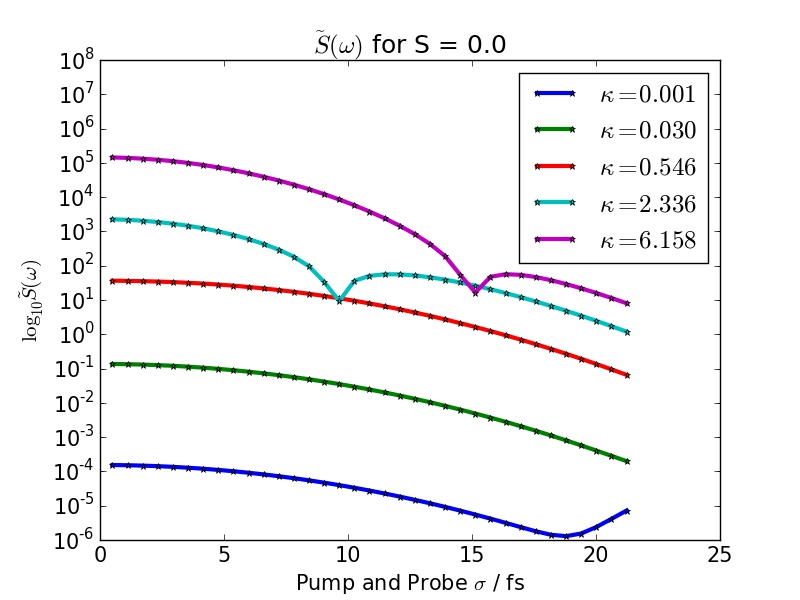
\includegraphics[width=0.5\textwidth]{images/s_omega_omegaSame_S0.jpeg}
   \caption{$\tilde{S}_{PP} ( \omega)$ for a system with no vibrational displacement and $\omega_{\gamma} = \omega_{\epsilon} = \omega = $ 640 cm$^{-1}$, for various values of $\kappa$.  The y-axis is log scaled because of the signal's fourth-order dependence on $\mu(x)$; small differences in $\kappa$ make very large differences in signal.  The dips is signal are an artifact of the system having the same ground and excited state vibrational frequency; they happen when the ground state bleach destructively intereferes with the excited state absorption.  In all of these systems, an experimenter using the proposed protocol would conclude that an electronic coherence exists in the system.}
	\label{fig:tunedZero}
\end{figure}

In \ref{fig:tunedZero} is this result for multiple vlaues of $\kappa$.  One can see quite clearly that there are oscillations in the vibrational frequency being induced and they are getting bigger as the pulse widths get smaller.  Problematically, this is precisely the signature of eletronic coherence suggested in \cite{allanWitness}.  This would mean, then, that an experiment would erroneously have diagnosed electronic coherence.  Although the non-constant transition dipole does induce a vibrational coherence on both the excited and ground state manifolds, the proposed experiment shows the signature of a electronic coherence when there is none.


\section{Interplay between Vibrational Coherence and Transition-Dipole Variation}
Perhaps, however, the situation is more complex in systems with vibrational coherences. That turns out not to be the case.  We first consider a monomer with a Huang-Rhys Parameter ($S$) of .2 and detuned vibrational frequencies of $\omega_e = .9 \omega_g$. and $\omega_g = 640 \text{cm}^{-1}$.  We  track both  the oscillations at $\omega_e$ and $\omega_g$.

\begin{figure}
   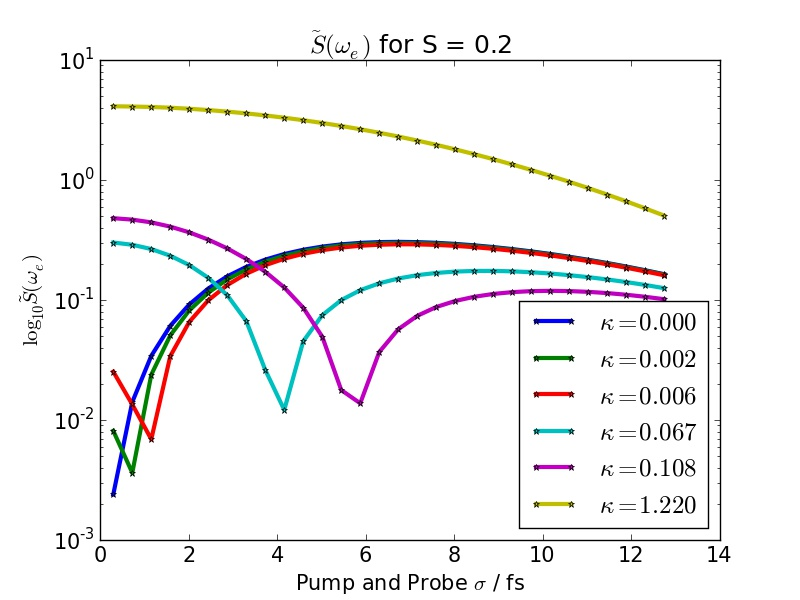
\includegraphics[width=0.5\textwidth]{images/s0point2_omega_e.jpg}
   \caption{$\tilde{S}_{PP} ( \omega_e)$ for various values of $\kappa$ in a system where S=0.2, $\omega_e = .9 \omega_g$. and $\omega_g = 640 \text{cm}^{-1}$.  }
	\label{fig:detunedMediumExcited}
\end{figure}

\begin{figure}
   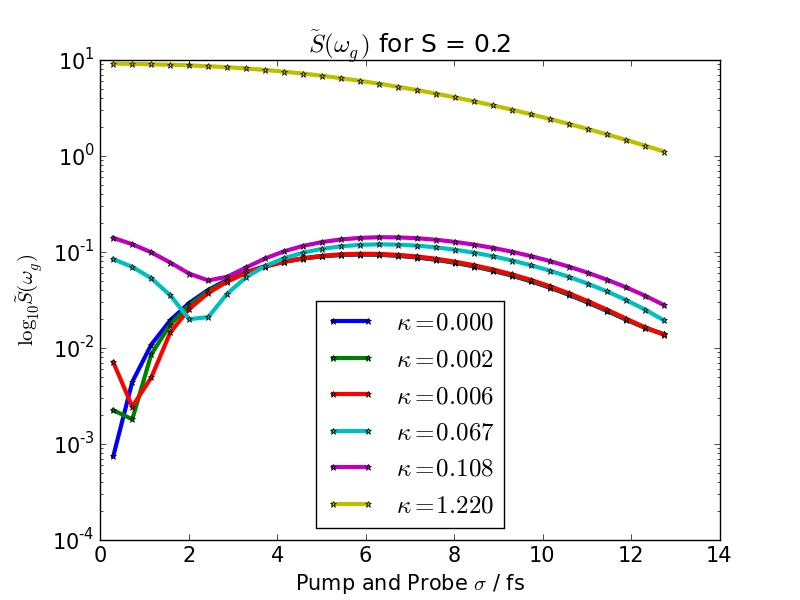
\includegraphics[width=0.5\textwidth]{images/s0point2_omega_g.jpg}
   \caption{$\tilde{S}_{PP} ( \omega_g)$ for various values of $\kappa$ in a system where S=0.2, $\omega_e = .9 \omega_g$. and $\omega_g = 640 \text{cm}^{-1}$.  }
	\label{fig:detunedMediumGround}
\end{figure}

In \ref{fig:detunedMediumExcited} we see clear problems emerging for even small values of $\kappa$.  For even the smallest investigated value of $\kappa$ in this system, should thin enough laser pulses be available, the conclusion according to \cite{allanWitness} would be that the system contains electronic coherence.  We also see similar issues in $\tilde{S} ( \omega_g)$ in \ref{fig:detunedMediumGround}, but they are of less import because $\tilde{S} ( \omega_g ) $ only captures oscillations in the ground state bleach terms, which decay proportional to $\sigma^2$ and not $\sigma$ like the  excited state absorption terms.

A Huang-Rhys parameter of .2, however, is rather far away from what values for strongly-coupled photosynthetic modes \cite{typicalStwo}.  If instead we look at S=.005, which is much closer in the range the experiment appears even more broken. [NEED SMALLER $\kappa$ VALUE?] %\cite{junkCitation} not working for some FUCKING reason?!!?!?

\begin{figure}
   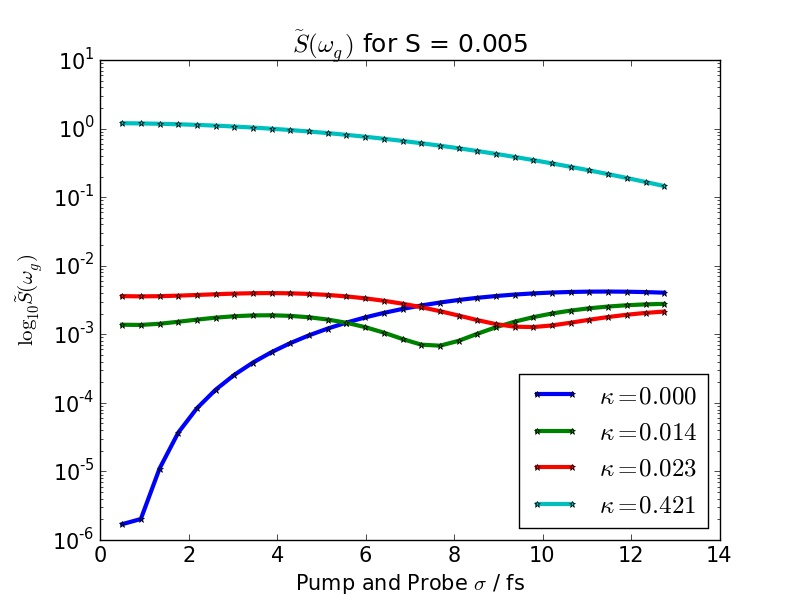
\includegraphics[width=0.5\textwidth]{images/s0point005_omega_g.jpg}
   \caption{$\tilde{S}_{PP} ( \omega_g)$ for various values of $\kappa$ in a system where S=0.005, $\omega_e = .9 \omega_g$. and $\omega_g = 640 \text{cm}^{-1}$.  }
	\label{fig:detunedSmallGround}
\end{figure}


\begin{figure}
   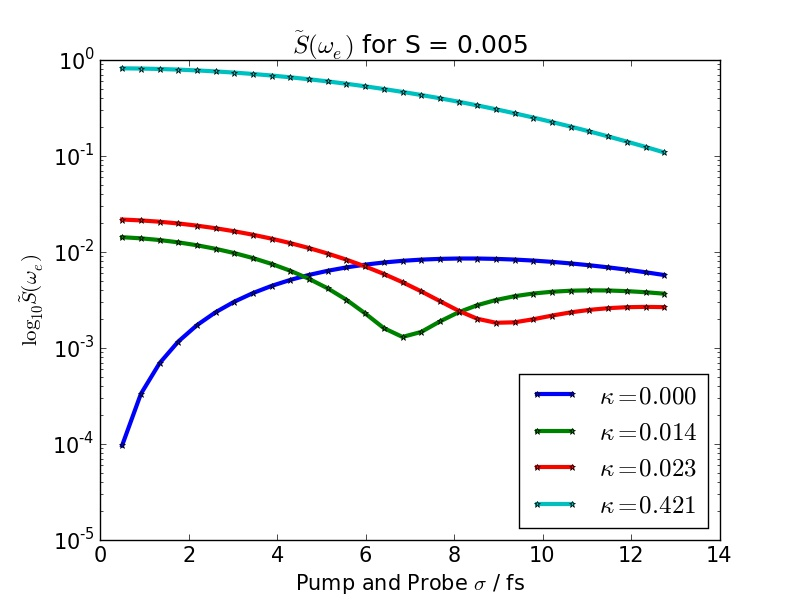
\includegraphics[width=0.5\textwidth]{images/s0point005_omega_e.jpg}
   \caption{$\tilde{S}_{PP} ( \omega_g)$ for various values of $\kappa$ in a system where S=0.005, $\omega_e = .9 \omega_g$. and $\omega_g = 640 \text{cm}^{-1}$.  }
	\label{fig:detunedSmallExcited}
\end{figure}
Once again for the amplitude at the excited state frequency in \ref{fig:detunedSmallExcited} for small values of $\kappa$, pump-probe spectra have oscillations which increase as the pulse widths get smaller.

\section{Non-Condonicity in Nature}
A fair question to ask would be: what kind of values of $\kappa$ would one expect to see in nature.  Reference \cite{photosyntheticKappa} predicted a $\kappa$ value of about 0.3 on a mode with a Huang-Rhys parameter of roughly 0.8, which is very close to our \ref{fig:detunedSmallGround} and \ref{fig:detunedSmallExcited} in the regime where the proposed experiment completely breaks without even a dip in signal before the .  Admittedly this was only on one mode, but without rigorous theory like they employed in the paper, it would be impossible to even guess whether a node had a transition dipole variation or not.

For another data-point of natural transition dipole variation, we calculated\cite{turbomolSoftware,Rappaport2005} the first order taylor expansion of the diatomic Iodine transition dipole, using density functional theory \cite{dft} from the ground state to the optically accessible BLANK state, using a DEF2-TZVP basis\cite{dftBasis} and the PBE0 functional\cite{dftFunctional}, which give (in atomic units):
\begin{align}
	\mu_{g \leftarrow e} &\approx -0.132477 - 0.04555 (x - \bar{x}_e )\\
	&\approx \mu_0 \left[ 1 + 0.3438(x - \bar{x}_e ) \right]\\
	\mu_{e \leftarrow g} &\approx -0.165270 - 0.0548235 (x - \bar{x}_g) \\
	&\approx \mu_0 \left[ 1 + 0.3317(x - \bar{x}_g ) \right]
\end{align}
or a $\kappa$ value of roughly .3 in both cases.  The Huang-Rhys paramter of Iodine is, however, quite large at 24.6 and dynamic spectroscopy results for it would not terribly applicable to determining whether there is electronic coherence in photosynthetic systems.  What this does seem to show, however, is that perhaps the Condon Approximation is not as firm as once thought.  We treat possible methods of detecting transition dipole variation in another paper(?)

\section{Conclustion}
We have shown that for small and hardly atypical linear variation in the transition dipole moment cause signatures in Pump-Probe spectroscopy that would be mistaken for an electronic coherence.
